\documentclass{beamer}
\usepackage{amsmath}
\usepackage{amssymb}
\usepackage{pgf}
\usepackage{tikz}
\usetikzlibrary{matrix}
\usetheme{boxes}
\newcommand{\fig}{figures}
\newcommand{\frnzplt}{FranzPlot }


\title[Curve e Sup. - Lab 1]{Curve e Superfici per il Design \\ Laboratorio - 1}
\author[Prof. Scotti]{Prof. Anna Scotti}
%\institute[dimat]{Long Inst.}
\date{2 Aprile 2019}

\begin{document}
\begin{frame}
\maketitle
\end{frame}
\section{Trasformazioni}
\begin{frame}
\frametitle{Rotazioni: Asse x}
\begin{equation}
R_x(\theta) = 
\begin{bmatrix}
1 & 0 & 0 \\
0 & \mbox{cos}(\theta) & - \mbox{sen}(\theta)\\
0 & \mbox{sen}(\theta) & \mbox{cos}(\theta)
\end{bmatrix}
\end{equation}
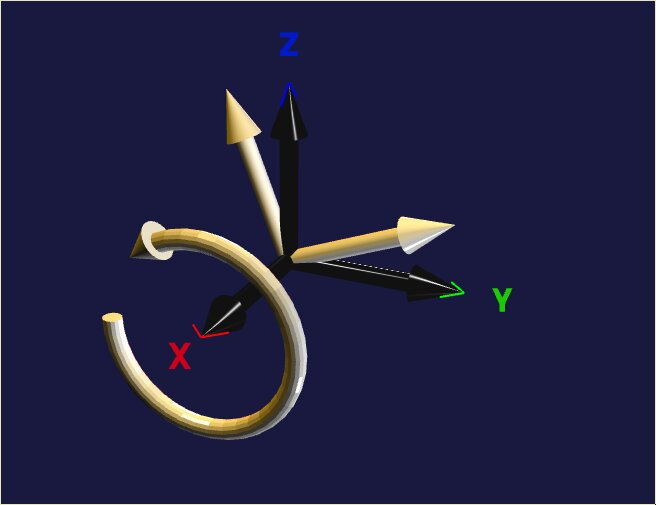
\includegraphics[width=0.6\textwidth]{\fig/rot_x.jpeg}
\end{frame}
\begin{frame}
\frametitle{Rotazioni: Asse y}
\begin{equation}
R_y(\theta) = 
\begin{bmatrix}
\mbox{cos}(\theta) & 0 & \mbox{sen}(\theta)\\
0 & 1 & 0 \\
-\mbox{sen}(\theta)& 0 & \mbox{cos}(\theta)
\end{bmatrix}
\end{equation}
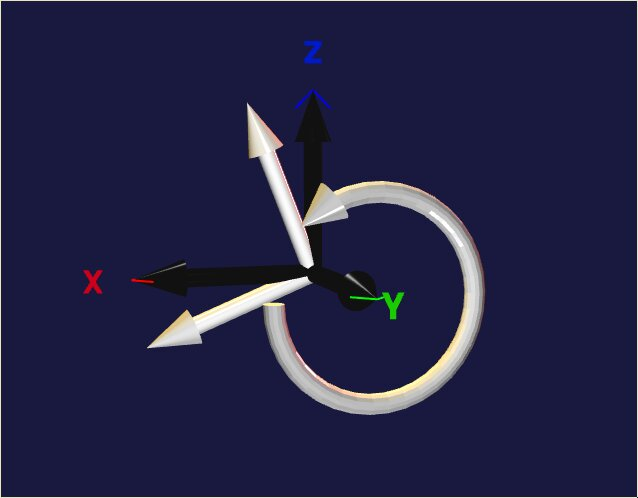
\includegraphics[width=0.6\textwidth]{\fig/rot_y.jpeg}
\end{frame}
\begin{frame}
\frametitle{Rotazioni: Asse z}
\begin{equation}
R_z(\theta) = 
\begin{bmatrix}
\mbox{cos}(\theta) & - \mbox{sen}(\theta) & 0\\
\mbox{sen}(\theta) & \mbox{cos}(\theta)   & 0\\ 
0 & 0 & 1 
\end{bmatrix}
\end{equation}
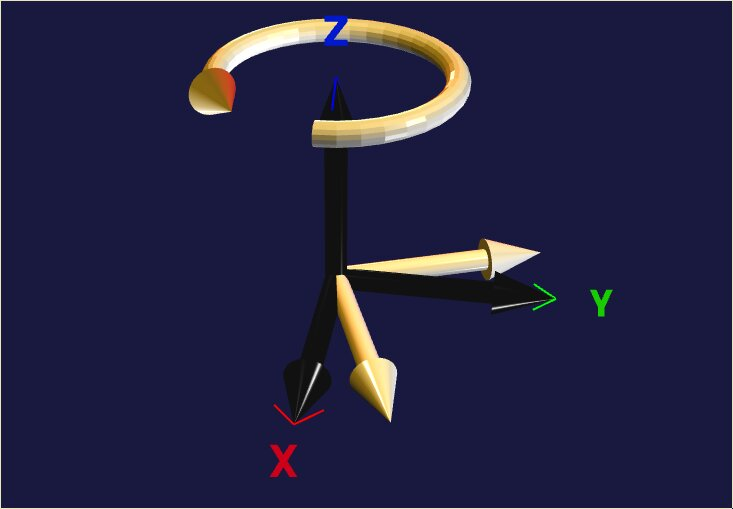
\includegraphics[width=0.6\textwidth]{\fig/rot_z.jpeg}
\end{frame}
%
\begin{frame}
\frametitle{Tagli}
\begin{columns}
\begin{column}{0.48\textwidth}
Taglio in direzione x sulle facce con normale y:
\begin{equation}
T_{xy}=\begin{bmatrix}
    1 & k_x & 0\\
    0 & 1   & 0\\
    0 & 0   & 1
    \end{bmatrix}
\end{equation}
\end{column}
\begin{column}{0.48\textwidth}
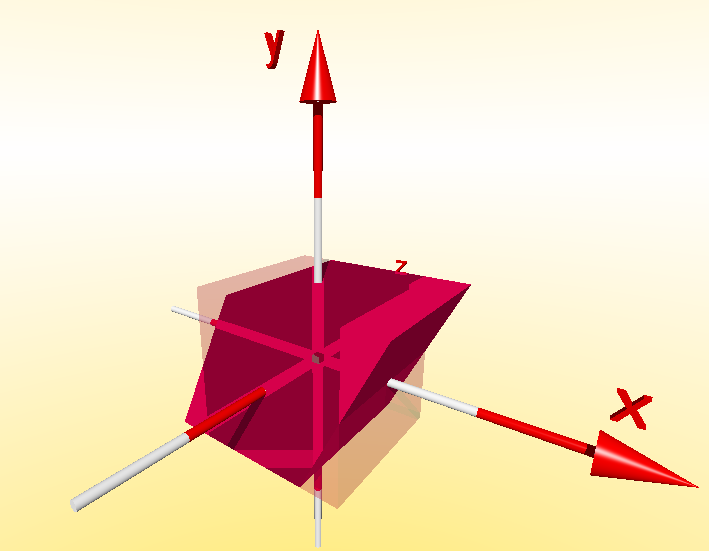
\includegraphics[width=0.8\textwidth]{\fig/cut_tx.png}
\end{column}
\end{columns}
%
\begin{columns}
\begin{column}{0.48\textwidth}
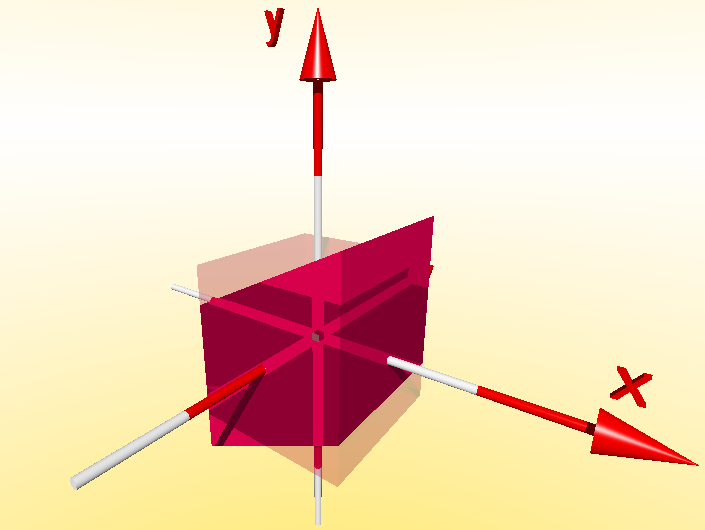
\includegraphics[width=0.8\textwidth]{\fig/cut_ty.png}
\end{column}
\begin{column}{0.48\textwidth}
Taglio in direzione y sulle facce con normale x:
\begin{equation}
T_{yx}=\begin{bmatrix}
    1   & 0 & 0\\
    k_y & 1 & 0\\
    0   & 0 & 1
    \end{bmatrix}
\end{equation}
\end{column}
\end{columns}
\end{frame}
%
\begin{frame}
\frametitle{Tagli[2]}
\begin{columns}
\begin{column}{0.48\textwidth}
Taglio in direzione z sulle facce con normale x:
\begin{equation}
T_{zx}=\begin{bmatrix}
    1 & 0 & 0\\
    0 & 1 & 0\\
    k_z & 0 & 1
    \end{bmatrix}
\end{equation}
\end{column}
\begin{column}{0.48\textwidth}
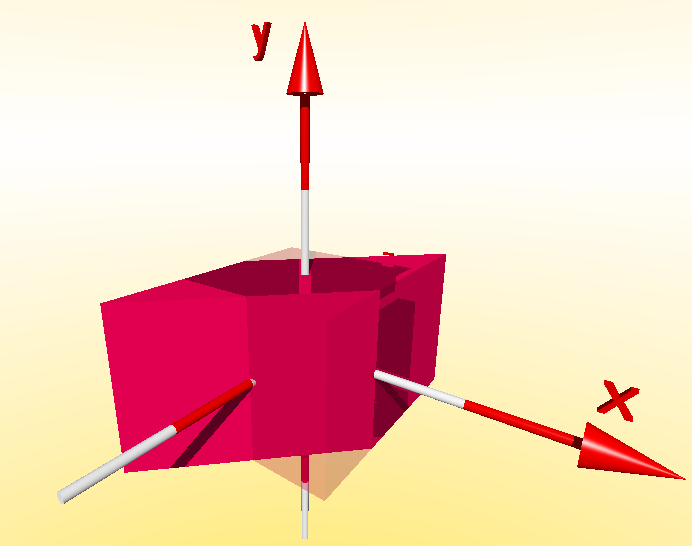
\includegraphics[width=0.8\textwidth]{\fig/cut_tz-x.png}
\end{column}
\end{columns}
%
%\begin{block}{}
\begin{columns}
\begin{column}{0.48\textwidth}
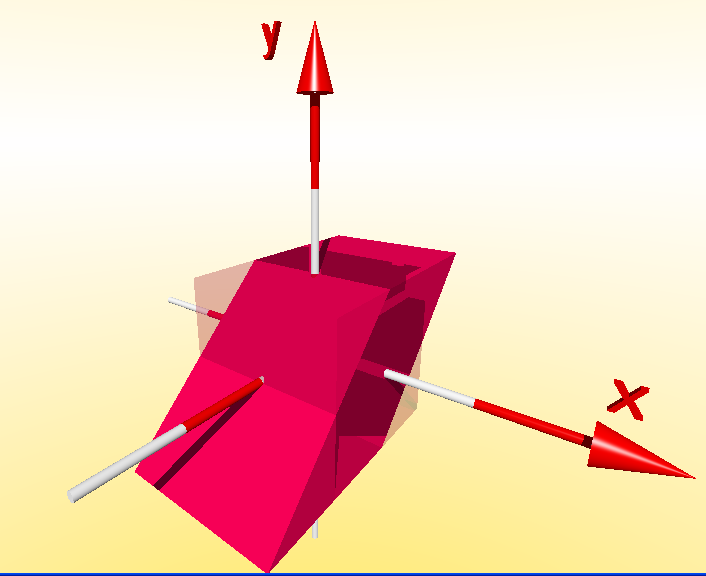
\includegraphics[width=0.8\textwidth]{\fig/cut_tz-y.png}
\end{column}
\begin{column}{0.48\textwidth}
Taglio in direzione z sulle facce con normale y:
\begin{equation}
T_{zy}=\begin{bmatrix}
    1 & 0 & 0\\
    0 & 1 & 0\\
    0 & k_z & 1
    \end{bmatrix}
\end{equation}
\end{column}
\end{columns}
%\end{block}
\end{frame}
%
\begin{frame}
\frametitle{Scalatura, Riflessione,Proiezione}
\begin{itemize}
\item Scalatura
\begin{equation}
S = \begin{bmatrix}
    S_x & 0 & 0\\
    0 & S_y & 0\\
    0 & 0 & S_z
    \end{bmatrix}
\end{equation}
\item Riflessione
\begin{equation}
F = \begin{bmatrix}
      1 & 0 & 0\\
      0 & 1 & 0\\
      0 & 0 & 1
    \end{bmatrix}
    -2~\begin{bmatrix}
    n_x \\
    n_y \\
    n_z
    \end{bmatrix} 
    ~\begin{bmatrix}
    n_x & n_y & n_z
    \end{bmatrix}
\end{equation}
\item Proiezione
\begin{equation}
 P = \begin{bmatrix}
      1 & 0 & 0\\
      0 & 1 & 0\\
      0 & 0 & 1
    \end{bmatrix}
    -\begin{bmatrix}
    n_x \\
    n_y \\
    n_z
    \end{bmatrix} 
    ~\begin{bmatrix}
    n_x & n_y & n_z
    \end{bmatrix}
\end{equation}
\end{itemize}
\end{frame}
%
\begin{frame}
\frametitle{Coordinate omogenee}
\begin{displaymath}
\begin{bmatrix}
a_{11} & a_{12} & a_{13} & t_1 \\
a_{21} & a_{22} & a_{23} & t_2 \\
a_{31} & a_{32} & a_{33} & t_3 \\
0      &    0   &  0     & 1 
\end{bmatrix}
~\begin{bmatrix}
x \\ y\\ z\\ 1
\end{bmatrix}
=  
\begin{bmatrix}
a_{11}x + a_{12}y + a_{13}z + t_1 \\
a_{21}x + a_{22}y + a_{23}z + t_2 \\
a_{31}x + a_{32}y + a_{33}z + t_3 \\
 1
\end{bmatrix}
\end{displaymath}
\end{frame}


\section{Il \frnzplt}
\begin{frame}
\frametitle{Il \frnzplt in breve}
\frnzplt nasce come strumento software specificamente come supporto per la didattica di questo corso.
\begin{itemize}
  \item \'E in grado di rappresentare attraverso un rendering superfici e curve parametriche.
  \item La creazione e la trasformazione degli oggetti rappresentati avviene attraverso la produzione di diagrammi (grafi).
  \item Ogni elemento del grafo ha una funzione specifica ed usualmente \`e legato ad uno o pi\`u elementi aggiuntivi.
  %\item Il documento di riferimento (WIP) del programma \`e disponibile su beep nella cartella taldeitali.
\item \frnzplt \`e al momento disponibile come eseguibile per Windows su Beep nella cartella FranzPlot-DCS. 
\end{itemize}
\end{frame}
\begin{frame}
\frametitle{Come avviare \frnzplt}
\begin{itemize}
\item Una volta scaricato l'eseguibile \texttt{franzplot.exe} e spostato nella
cartella dove si intende lavorare (possibilmente sul disco locale - nei
computed del laboratorio informatico \`e usualmente indicato con Z:), \`e
possibile eseseguirlo normalmente per avviare il programma.  
\item Nel caso si
presentassero problemi di visualizzazione, potrebbe rivelarsi necessario
scaricare dalla stessa cartella BeeP anche il file \texttt{launcher.bat} ed eseguirlo.
\end{itemize}
\end{frame}

\section{Esercizi}
\begin{frame}
\frametitle{Esercizio 1: prendere familiarit\`a con \frnzplt}
\frnzplt ha a disposizione una piccola libreria di figure geometriche primitive, figure solide gi\`a costruite, accessibile attraverso il menu: \texttt{Geometries} $\rightarrow$\texttt{Primitive}.
\begin{itemize}
\item Disegnare un cilindro con asse parallelo a z ed altezza 1.
\begin{itemize}
\item \textit{Elementi da utilizzare:} \texttt{Geometries}$\rightarrow$ \texttt{Primitives}, \texttt{Geometry Renderer}.
\end{itemize}
\item Effettuare uno scaling con $S_x =2$, $S_y=1$, $S_z=0.5$.
\begin{itemize}
\item \textit{Elementi aggiuntivi da utilizzare:} \texttt{Transformations}$\rightarrow$ \texttt{Generic Matrix} \textit{e} \texttt{Transformations}$\rightarrow$\texttt{Transform}
\end{itemize}
%\item Traslare l'oggetto ottenuto di un vettore a scelta parallelo ad y.
\end{itemize}
\end{frame}
\begin{frame}
\frametitle{Esercizio 1 - i}
\begin{center}
\begin{tikzpicture}
\node(img1){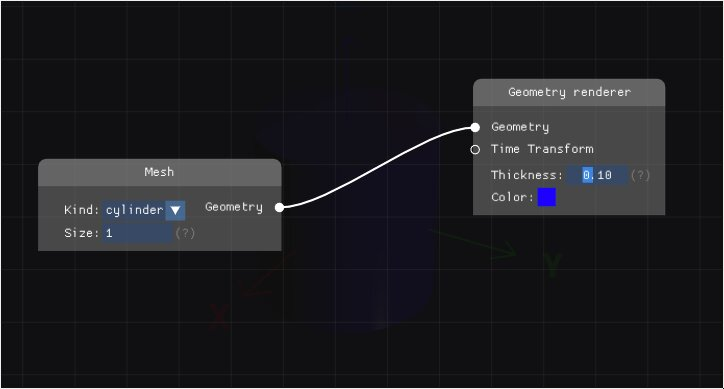
\includegraphics[width=0.7\textwidth]{\fig/l1_cylinder_ex.jpeg}};
\node(img2) at (img1.north west){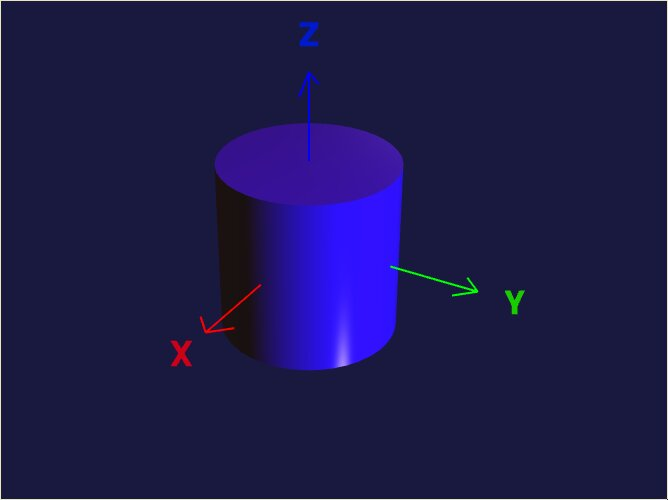
\includegraphics[width=0.4\textwidth]{\fig/l1_cylinder_ex_img.jpeg}};
\end{tikzpicture}
\end{center}
\end{frame}
\begin{frame}
\frametitle{Esercizio 1 - ii}
\begin{center}
\begin{tikzpicture}
\node(img1){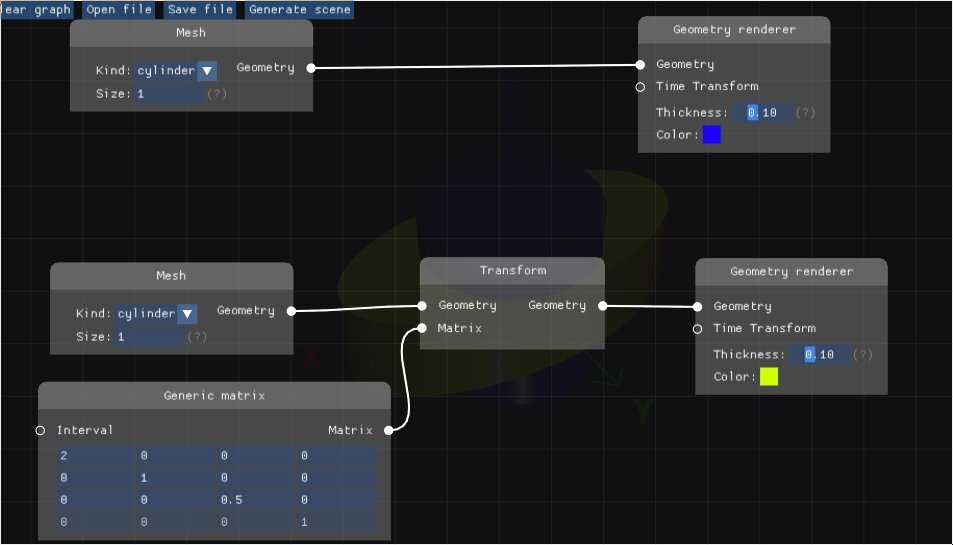
\includegraphics[width=0.7\textwidth]{\fig/l1_cylinder_ex_graph2.jpeg}};
\node(img2) at (img1.north west){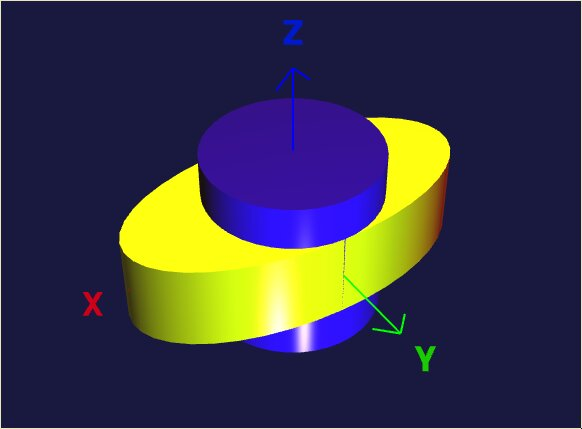
\includegraphics[width=0.4\textwidth]{\fig/l1_cylinder_ex_graph2_img.jpeg}};
\end{tikzpicture}
\end{center}
\end{frame}

\begin{frame}
\frametitle{Esercizio 2: Identificare una trasformazione}
\begin{itemize}
\item Disegnare un  cubo centrato sull'origine, con lati di misura 2 (notare
che nella primitiva \`e possbile fissare un parametro che influenza la
dimensione dell'oggetto).  
\item Applicare al cubo la seguente matrice: 
\begin{displaymath}
A = \begin{bmatrix}
    1 & 0 & 1\\
    0 & 1 & 0\\
    0 & 0 & 1
    \end{bmatrix}
\end{displaymath}
\item Di che trasformazione si tratta? Qual'\`e il volume del cubo deformato?
\end{itemize}
\end{frame}
%
\begin{frame}
\frametitle{Esercizio 2 - i}
\begin{center}
\begin{tikzpicture}
\node(img3){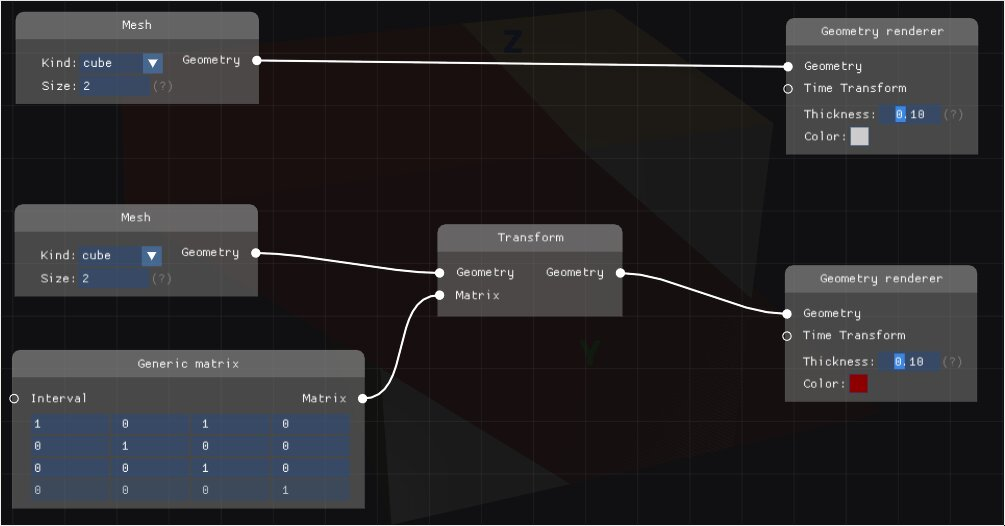
\includegraphics[width=0.7\textwidth]{\fig/l1_es2_graph.jpeg}};
\node(img4) at (img3.south west){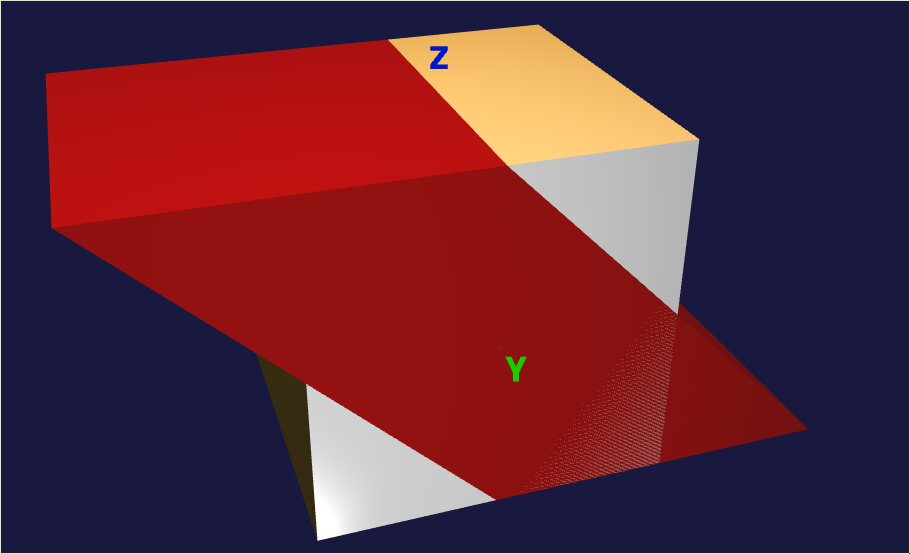
\includegraphics[width=0.4\textwidth]{\fig/l1_es2_img.jpeg}};
\end{tikzpicture}
\end{center}
\end{frame}
% ESEMPIO TRASLAZIONE (SENZA SPIEGAZIONE ) CON TRASFORMAZIONE NEL TEMPO
\begin{frame}
\frametitle{Esercizio 3: Trasformazioni tempo dipendenti con \frnzplt}
\begin{itemize}
\item Riprendendo il grafo dell'Es.1, aggiungere al cilindro deformato una trasformazione nel tempo del tipo:
\begin{displaymath}
A = \begin{bmatrix}
    1 & 0 & 0 & 0 \\
    0 & 1 & 0 & 0 \\
    0 & 0 & 1 & t \\
    0 & 0 & 0 & 1
    \end{bmatrix}
\end{displaymath}
\item Utilizzare l'elemento \texttt{Transformations} $\rightarrow$ \texttt{Time Transform} \textit{Attenzione: l'uso della lettera t per indicare la variabile temporale in questa matrice \`e mandatoria.}
\end{itemize}
\begin{center}
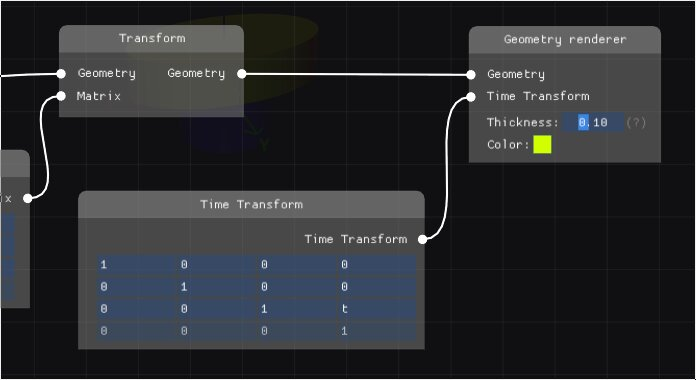
\includegraphics[width=0.4\textwidth]{\fig/l1_es3_graph.jpeg}
\end{center}
\end{frame}
%%%
\begin{frame}
\frametitle {Esercizio 4 - Riflessione}
\begin{itemize}
\item Creare un oggetto 'dado' utilizzando il comando Primitive, con fattore di scala 0.5.
\item Traslare il centro dell'oggetto in   $\langle 2,1,0\rangle$  (combinando gli elementi \texttt{Transformations} $\rightarrow$ \texttt{Translation Matrix} e \texttt{Vector}).  
\item Riflettere l'oggetto rispetto al piano con normale $\textbf{N}=[1,1,0]^T$.
\item Rappresentare il piano di riflessione.
\end{itemize}
\end{frame}
\begin{frame}
\frametitle {Esercizio 4 - i - La matrice di trasformazione}
Come prima cosa, occorre normalizzare $\textbf{N}$.
\begin{displaymath}
\sqrt{\mathbf{N} \cdot \mathbf{N}} =\sqrt{ N_x^2+N_y^2+N_z^2}=\frac{\sqrt{2}}{2}
\end{displaymath}
Applicando la formula per la trasformazione di `proiezione':
\begin{displaymath}
\begin{bmatrix}
1 & 0 & 0 \\
0 & 1 & 0 \\ 
0 & 0 & 1 
\end{bmatrix}
- 2~ \left(\frac{\sqrt{2}}{2}\right)^2
\begin{bmatrix}
1 \\
1 \\ 
0 
\end{bmatrix}
\begin{bmatrix}
1 & 1 &  0
\end{bmatrix}
= 
\begin{bmatrix}
1 & 0 & 0 \\
0 & 1 & 0 \\ 
0 & 0 & 1 
\end{bmatrix}
-
\begin{bmatrix}
1 & 1 & 0 \\
1 & 1 & 0 \\ 
0 & 0 & 0 
\end{bmatrix}
\end{displaymath}
{\color[rgb]{0.1,0,1}
\begin{displaymath}
=
\begin{bmatrix}
0  & -1 & 0 \\
-1 &  0 & 0 \\ 
0  &  0 & 1 
\end{bmatrix}
\end{displaymath}
}

\end{frame}
\begin{frame}
\frametitle{Esercizio 4 - ii - L'oggetto riflesso}
\begin{center}
\begin{tikzpicture}
\node(img1){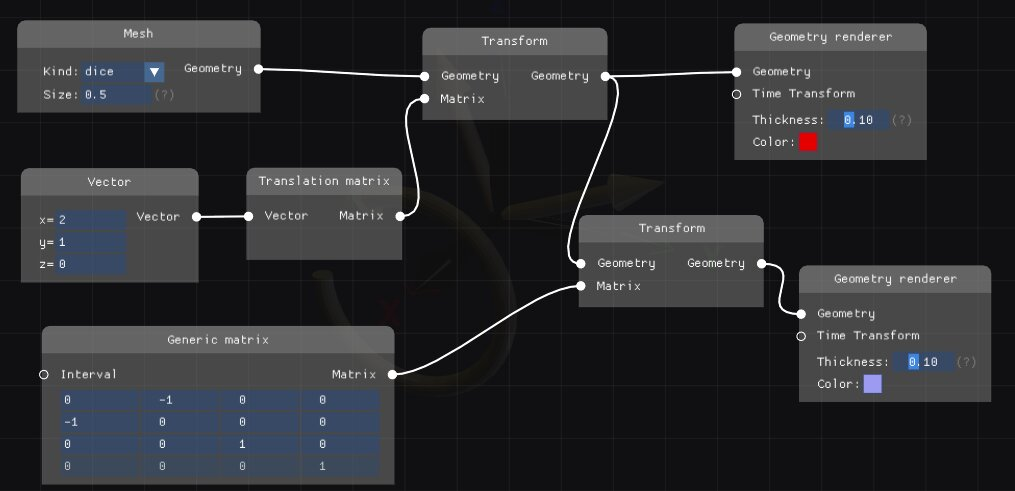
\includegraphics[width=\textwidth]{\fig/l1_reflection_graph1.jpeg}};
%\node(img2) at (img1.north west){\includegraphics[width=0.4\textwidth]{\fig/snapcode_3-3.png}};
\end{tikzpicture}
\end{center}
\end{frame}
\begin{frame}
\frametitle{Esercizio 4 - iii - Il piano}
\begin{center}
\begin{tikzpicture}
\node(img1){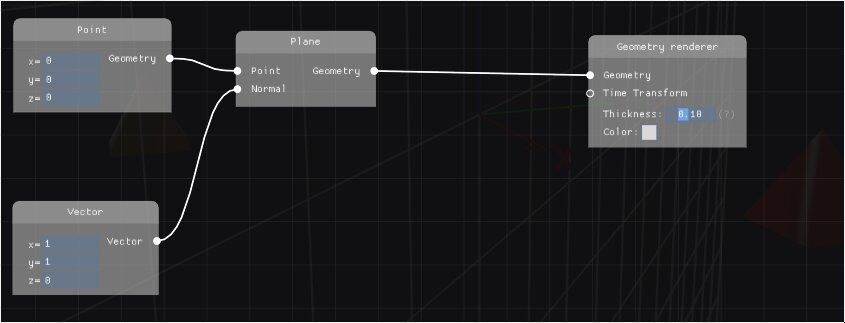
\includegraphics[width=\textwidth]{\fig/l1_reflection_graph2.jpeg}};
%\node(img2) at (img1.north west){\includegraphics[width=0.4\textwidth]{\fig/snapcode_3-3.png}};
\end{tikzpicture}
\end{center}
\end{frame}
\begin{frame}
\frametitle{Esercizio 4 - iv}
\begin{center}
\begin{tikzpicture}
\node(img1){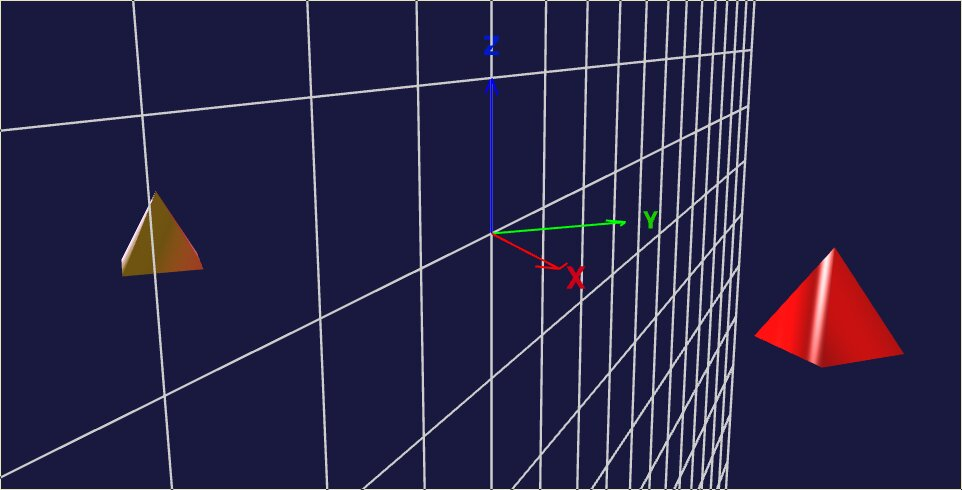
\includegraphics[width=\textwidth]{\fig/l1_reflection_img.jpeg}};
%\node(img2) at (img1.north west){\includegraphics[width=0.4\textwidth]{\fig/snapcode_3-3.png}};
\end{tikzpicture}
\end{center}
\end{frame}

\begin{frame}
\frametitle{Per Casa: Proiezioni ortogonali}
\begin{columns}
\begin{column}{0.32\textwidth}
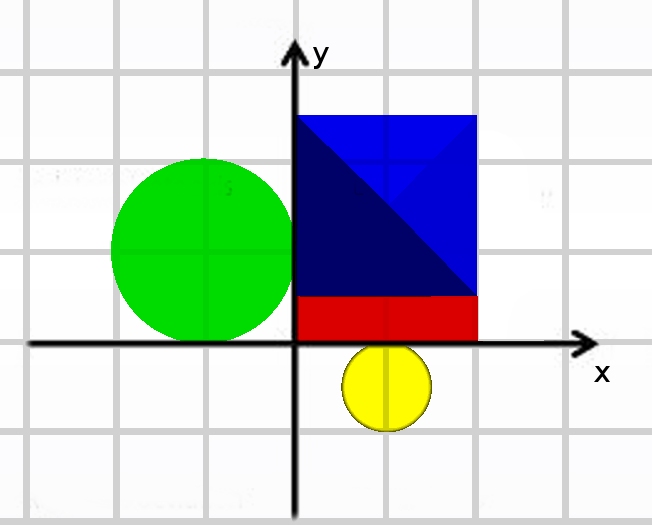
\includegraphics[width=\textwidth]{\fig/proj1.png}
\end{column}
\begin{column}{0.32\textwidth}
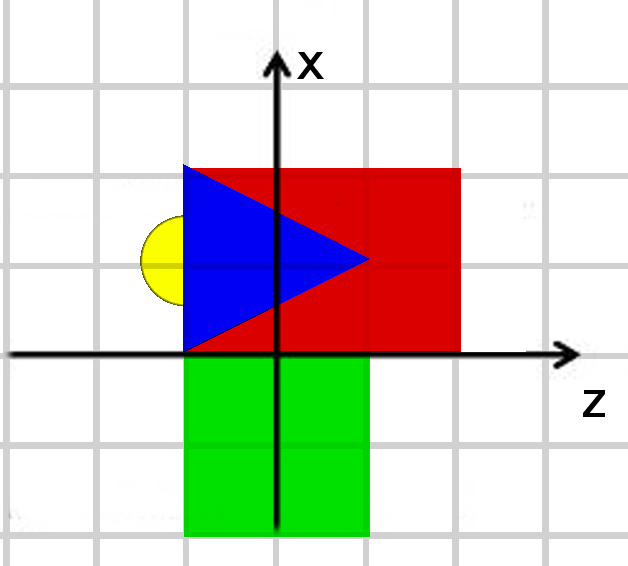
\includegraphics[width=\textwidth]{\fig/proj2.png}
\end{column}
\begin{column}{0.32\textwidth}
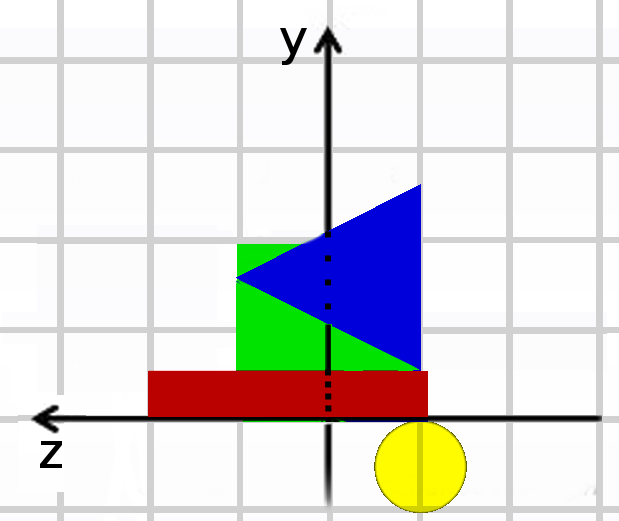
\includegraphics[width=\textwidth]{\fig/proj3.png}
\end{column}
\end{columns}
\vspace{20pt}
Creare un'organizzazione di oggetti le cui proiezioni sui piani cartesiani riproducono le figure sovrastanti.
\end{frame}

\end{document}

